\section{Uniform Rational Basis Splines}

\subsection{Introduction to URBS}


\subsection{Design Rationale}


The decision to use a method of restricting and structuring the input curve type was made for several reasons. 

Firstly the structure that a spline based representation gives to the input data gives natural compression for that data, as compared to storing the location of each individual point upon the desired curve. This allows for easy storage and manipulation of input curves by the GUI program. 

Secondly the restriction of the curves to splines of the 3rd order ensures that the parametrised curve $\textbf{q}(s)$ has the property of being twice differentiable;
\begin{align*}
\textbf{q}(s) \in \mathbb{C}^2
\end{align*}
If this were not the case, the path velocity could not be be guaranteed to be continuous. The plant would then require infinite acceleration at those discontinuities in order to travel the path at any speed. 

Finally the parametrisation of the curve $\textbf{q}(s)$, allows us to easily retrieve the path velocity $\textbf{q}'(s) = \frac{dq(s)}{ds}$ and path acceleration $\textbf{q}''(s) =  \frac{d^2q(s)}{ds^2}$ along any point on the curve. This is useful in calculating the force along an axis required for any given $\dot{s}(t)$

Given this rationale, 3rd order Uniform Rational Basis Splines (URBS) were used as the curve data structure. The general weighting structure of an URBS is the same for each and every curve, given the uniformity of their knots. URBS are a specific case of the widely used Non-Uniform Rational Basis Splines (NURBS), where the knot vector contains only evenly spaced knots. The knot vector defines one or greater knot spans, which thereon define the rise and decay of weighting for a series of control points, as can be seen in Fig~\ref{fig:nurbsBasis} 

\begin{figure}  
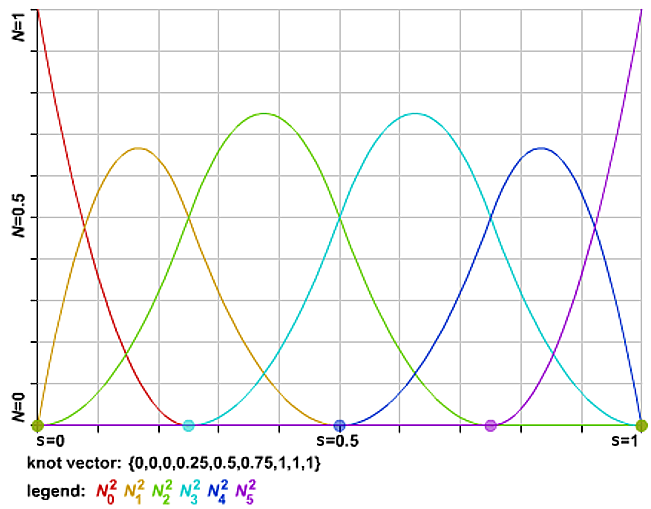
\includegraphics[width=\textwidth]{figures/optimisation/nurbsBasis.png}
\caption[3rd order (Quadratic) URBS basis splines]{ These splines represent the weighting of each of the six control points $\textbf{N} \in \{\textbf{N}_0^2, \textbf{N}_1^2 \cdots \textbf{N}_5^2\}$, with the parameter $s \in [0, 1].$ \cite{website:nurbsDemo}  
\label{fig:nurbsBasis}}
\end{figure}

For the class of 3rd order URBS used, weighting coefficients that multiply each of the control points quadratically shift across the domain of $s \in [0, 1]$. This brings consecutive control points into prominence evenly as the path parameter is traversed. Each point on the curve consists of a linear combination of the control points $\textbf{N}_i^2, \textbf{N}_{i-1}^2, \textbf{N}_{i-2}^2$, defined by the weighting of their basis function at that point.

When the $s$ parameter passes a knot value, such as $s = 0.5$ in Fig~\ref{fig:nurbsBasis}, it signifies that one control point no longer has influence over the position of the path and the next control point will begin to rise in weighting. Note that there are three repeated knots at the beginning and end of a curve. These knots make sure that the curve terminates at the location of the first and last control point. They also ensure that the weighting functions have defined values throughout the recursive calculations.

In this way each point on the curve is defined by a linear combination of three control points and each control point has weighted influence over a similar sized domain on $s$. The weightings for each control point can be determined given the knot vector, which is uniform and defined when one is given the number of control points a curve will contain.

The knot vector can be obtained by applying the following algorithm, where $N$ is defined as the number of control points.
\begin{align*}
K_N &= \left[0, 0,  \frac{n_0 - 3}{N-2}, \frac{n_1 - 3}{N-2}, \cdots ,\frac{n_i - 3}{N-2}, 1, 1\right]\\  
\textit{s.t. }n_i &\in \left[3, N+1\right]
\\ N &\geq 3
\\n_i, N &\in \mathbb{Z}
\end{align*}

A knot vector for the case when $N = 6$ can be seen in Fig~\ref{fig:nurbsBasis}.

The knot vector can be calculated when one is given the number of control points of a curve. Subsequently we can use the recursive definition of the URBS basis function to calculate the the control point weightings at any given $s \in [0, 1] \therefore s \in [K_3, K_{N+1}]$
\begin{align*}
W_{i,d}(s) &=   \frac{s - K_i}{K_{i+d} - K_i}W_{i,d-1}(s)  +  \frac{K_{i + d + 1} - s}{K_{i + d + 1} - K_{i+1}}W_{i+1,d-1}(s)\\
W_{i,0}(s) &= \begin{cases}
   1 & \text{if } K_i \leq s < K_{i+1} \\
   0 & \text{otherwise}
  \end{cases}
\end{align*}
Where $K_i$ is the knot at index $i$ and $d$ is the dimension of the URBS curve.

For the cases where the multiplying fractions result in $\frac{0}{0}$, we take the result to be $0$.

When the URBS curve is of dimension 2 the line equation for $q_i(s) = q(s)\bigm|_{K_i \leq s < K_{i+1}}$ results in the following definition \cite{website:nurbsExplain};
\begin{align*}
q_i(s) = \textbf{N}_i^2W_{i,2}(s) + \textbf{N}_{i-1}^2W_{i-1,2}(s) + \textbf{N}_{i-2}^2W_{i-2,2}(s)
\end{align*}
Where $\textbf{N}_i^2 = \begin{bmatrix}
x_i\\y_i
\end{bmatrix}$ is the $i$th control point and $W_{i,2}(s)$ is the second order basis weighting corresponding to that control point. 
For details of the derivation of $W_{i,2}(s)$, please see Appendix A.

Given the piecewise form of the line, one can easily take the derivative of $q(s)$ with respect to $s$ and obtain the path velocity $q'(s)$ and path acceleration $q''(s)$ utilising the same control points and knot indexes.
 
URBS were used over their better known cousins Non-Uniform Rational Basis Splines (NURBS) due to the even distribution of knots given by URBS ensuring that the optimisation solution we utilised broke the problem into even parts. If knots were allowed to be closer together in sections, it would mean that our solution technique would need to take this into account when dividing up the path space into discrete chunks. Using URBS rather than NURBS mitigates this problem at the cost of requiring more control points to specify curves with finer detail.